%%%%%%%%%%%%%%%%%%%%%%%%%%%%%%%%%%%%%%%%%
% University/School Laboratory Report
% LaTeX Template
% Version 3.1 (25/3/14)
%
% This template has been downloaded from:
% http://www.LaTeXTemplates.com
%
% Original author:
% Linux and Unix Users Group at Virginia Tech Wiki 
% (https://vtluug.org/wiki/Example_LaTeX_chem_lab_report)
%
% License:
% CC BY-NC-SA 3.0 (http://creativecommons.org/licenses/by-nc-sa/3.0/)
%
%%%%%%%%%%%%%%%%%%%%%%%%%%%%%%%%%%%%%%%%%

%----------------------------------------------------------------------------------------
%	PACKAGES AND DOCUMENT CONFIGURATIONS
%----------------------------------------------------------------------------------------

\documentclass{article}

\usepackage[version=3]{mhchem} % Package for chemical equation typesetting
\usepackage{siunitx} % Provides the \SI{}{} and \si{} command for typesetting SI units
\usepackage{graphicx} % Required for the inclusion of images
\usepackage{natbib} % Required to change bibliography style to APA
\usepackage{amsmath} % Required for some math elements 
\usepackage[utf8]{inputenc}
\usepackage[margin=1.2in]{geometry}

\setlength\parindent{0pt} % Removes all indentation from paragraphs

% \renewcommand{\labelenumi}{\alph{enumi}.} % Make numbering in the enumerate environment by letter rather than number (e.g. section 6)

\renewcommand{\figurename}{Figura}
\renewcommand{\tablename}{Tabla}
\renewcommand\refname{Referencias}

%\usepackage{times} % Uncomment to use the Times New Roman font

%----------------------------------------------------------------------------------------
%	DOCUMENT INFORMATION
%----------------------------------------------------------------------------------------

\title{M\'etodos num\'ericos para la Ciencia e Ingenier\'ia \\ Tarea 5: Integraci\'on de Ecuación de Poisson 2D} % Title

\author{Felipe Toledo Bittner} % Author name

\date{\today} % Date for the report

\begin{document}

\maketitle % Insert the title, author and date

%----------------------------------------------------------------------------------------
%	SECTION 1
%----------------------------------------------------------------------------------------

\section{Introducción}

En electrostática la Ecuación de Poisson (\ref{eq:eq_poisson}) describe el potencial eléctrico $V$ a partir de la distribución espacial de carga libre $\rho$ en el sistema, con $\epsilon$ una constante del medio físico:

\begin{equation}
  \nabla^2 V(\vec{x}) = \frac{-\rho(\vec{x})}{\epsilon}
  \label{eq:eq_poisson}
\end{equation}

Si la distribución de las cargas eléctricas es muy compleja, resolver esta ecuación de forma analítica puede ser imposible. Debido a que en experimentos reales la carga no necesariamente se ordena de forma sencilla, se vuelve necesario el estudiar e implementar métodos numéricos que permitan resolver esta ecuación para mayor diversidad de geometrías.

En este trabajo se implementa un programa que permite resolver la ecuación de Poisson en dos dimensiones para una geometría de difícil integración analítica utilizando el algoritmo de relajación.

\subsection{Descripción del problema}

Se debe integrar la Ecuación de Poisson en 2D para una caja rectangular con los siguientes requerimientos:

\begin{enumerate}
  \item Dimensiones de 10 [cm] x 15 [cm]
  \item Condiciones de borde: 
  \begin{enumerate}
    \item Potencial $V = 0$ en todo el perímetro.
    \item C.B. derivativa: $\frac{dV}{dy} = 1$ en la línea $x = [-3:3]$; $y = -5.5$ [cm] respecto al centro de la caja.
  \end{enumerate}
  \item Letra "F" de carga total $1[C]$ encerrada en un rectángulo centrado de 5 [cm] x 7 [cm].
\end{enumerate}


\section{Implementación}

\subsection{Software}

La solución del problema se realizó implementando los archivos \emph{main.py} y \emph{box.py}.

El archivo \emph{box.py} es una clase que contiene todos los métodos necesarios para operar y simular el problema solicitado, incluyendo elementos que permiten operar con coordenadas en centímetros, dibujar cargas en la caja, escribir condiciones de borde incluyendo derivativas e integrar la Ecuación de Poisson.

Por otro lado el archivo \emph{main.py} es el archivo ejecutable. Se utiliza para crear objetos caja, definir sus parámetros, iniciar las operaciones de cálculo y presentar los resultados.

La caja se representa usando dos matrices con resolución $h=0.1$ [cm]. Una matriz se utiliza para almacenar los valores de voltaje y condiciones de borde y la otra almacena la distribución de carga en el espacio. En la Figura (\ref{fig:situacion_inicial})

Esta solución posee la ventaja de almacenar la carga de inmediato en memoria. Así, para calcular el potencial en cada punto basta leer su casilla correspondiente de la matriz de carga para obtener su valor local. Con ellos se simplifica la implementación del programa y se adquiere más velocidad al privilegiar un acceso directo a memoria sobre otras alternativas como consulta de índices o árboles de decisión.

\begin{figure}
  \centering
  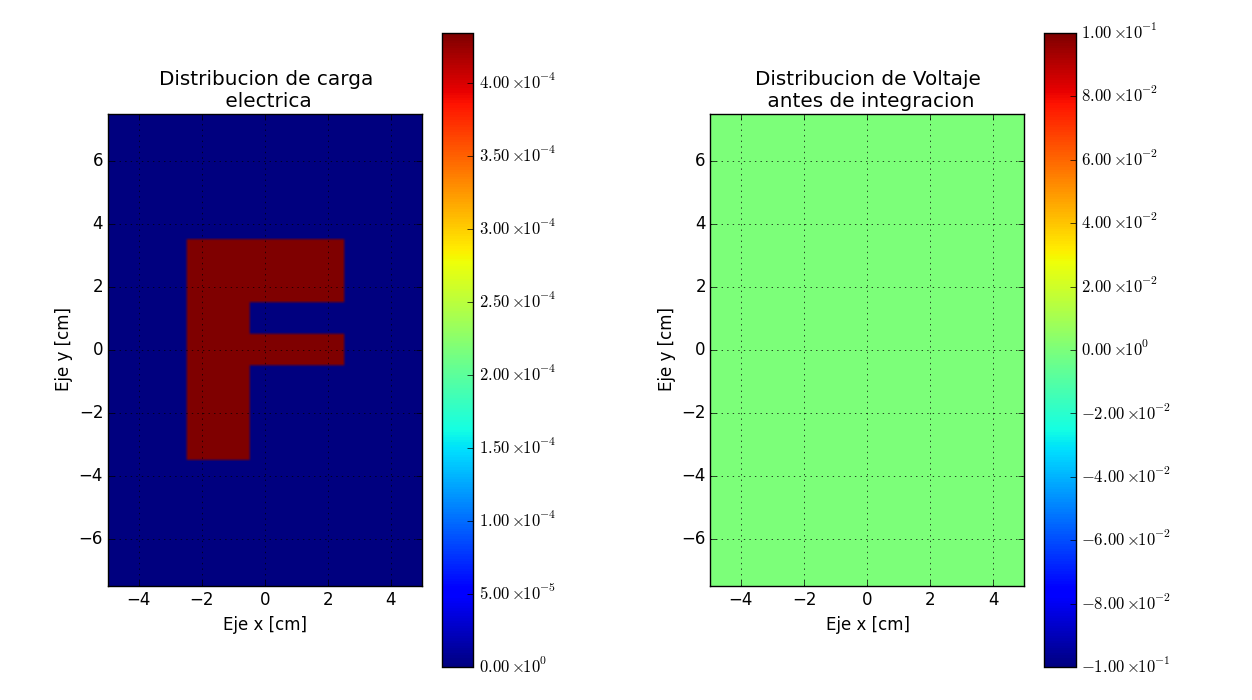
\includegraphics[scale=0.5]{images/situacion_inicial.png}
  \caption{Situacion inicial de las cajas de carga y voltaje. Se observa la letra 'F' dibujada en la caja de carga y las condición $V=0$ en todo el borde de la caja de potencial. Las unidades de carga son Coulomb y las de potencial, Voltaje.}
  \label{fig:situacion_inicial}
\end{figure}


\subsection{Algoritmo de relajación en 2D}
\label{sec:algoritmo}

El algoritmo de relajación consiste en calcular el valor de cada punto de una matriz usando los adyacentes durante sucesivas iteraciones, deteniéndose cuando se alcanza convergencia. Por convergencia se entiende el instante en que la diferencia entre dos iteraciones es menor a una determinada tolerancia para todos los puntos. En el caso de la ecuación de poisson, cada iteración del algoritmo de relajación calcula el voltaje de la celda $(i, j)$ usando la ecuación (\ref{eq:relajacion_poisson}). Para resaltar el efecto de las cargas se escoge $\epsilon = 5\cdot10^{-4}$ [F/m].

\begin{equation}
  V_{i,j}^{next} = \frac{1}{4} (V_{i+1,j} + V_{i-1,j} + V_{i,j+1} + V_{i,j-1} + h^2 \frac{\rho_{i,j}}{\epsilon}) 
  \label{eq:relajacion_poisson}
\end{equation}

En el programa se implementa una modificación a este algoritmo, que se puede observar en la fórmula (\ref{eq:relajacion_poisson_mejorada}). Con ésta se aprovecha que el cálculo de dos de los términos de la siguiente iteración se realizaron con anterioridad, que junto con el nuevo parámetro w permiten acelerar la convergencia.

\begin{equation}
  V_{i,j}^{next} = (1 - w)V_{i,j} + \frac{w}{4}(V_{i+1,j} + V_{i-1,j}^{next} + V_{i,j+1} + V_{i,j-1}^{next} + h^2 \rho_{i,j})
  \label{eq:relajacion_poisson_mejorada}
\end{equation}

Se escoge una tolerancia de $10^{-7}$ para determinar la finalización del algoritmo. Si se realizan más de 800 iteraciones se asume que no hay convergencia bajo los parámetros entregados y se interrumpe la ejecución.

\subsection{Condición de borde derivativa}

Para implementar la condición de borde derivativa se discretiza la derivada $\frac{dV}{dy} = 1$, quedando:

\begin{equation}
  \dfrac{(y_{i,j_0 + 1} - y_{i,j_0})}{h} = 1 \rightarrow y_{i,j_0 + 1} = h + y_{i,j_0}
\end{equation}

Donde $j_0$ es el índice de la casilla inmediatamente inferior a la línea $y = -5.5$ [cm], y los $i$ corresponden a los elementos ubicados en $x = [-3:3]$ [cm]. Luego de cada iteración del algoritmo de relajación se impone nuevamente la condición de borde, recalculando $y_{i,j_0 + 1}$. Como $h=0.1$, la línea queda justo entre dos casillas, evitándose que queden puntos sobre ella. Esto simplifica la implementación ya que no hay que calcular potencial justo encima de la condición de borde.


\section{Resultados}

Los resultados del algoritmo de cálculo pueden verse en la Figura (\ref{fig:volt_calculado}). Como se indicó en la sección \ref{sec:algoritmo}, se escoge un $\epsilon$ tal que el potencial causado por las cargas pueda apreciarse junto a la condición de borde.

\begin{figure}
  \centering
  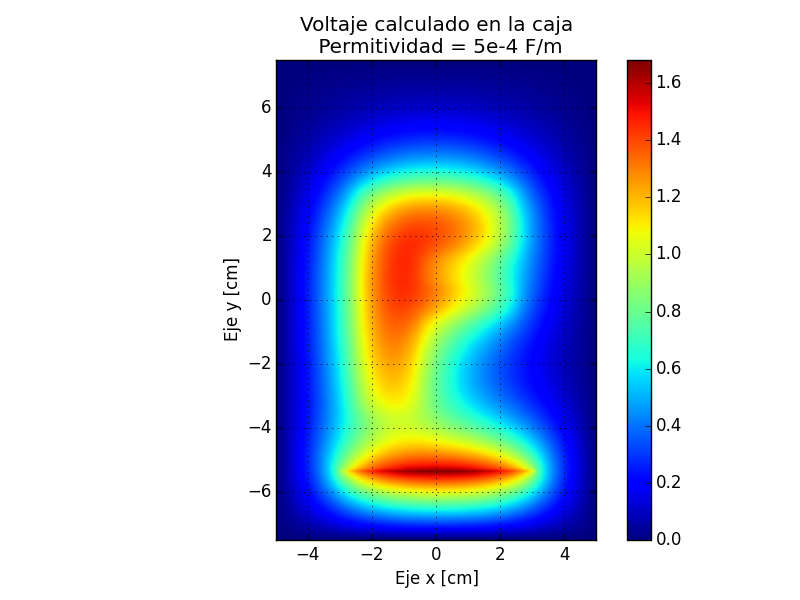
\includegraphics[scale = 0.7]{images/volt_calculado}
  \caption{Resultado del algoritmo de integración. Se observa claramente el efecto de la distribución de las cargas y las condiciones de borde en el potencial.}
  \label{fig:volt_calculado}
\end{figure}

\section{Conclusiones}

El algoritmo de relajación ha mostrado ser una herramienta simple y bastante eficaz para resolver el problema de integración de la ecuación de Poisson. Se debe notar que si se utilizase una distribución de carga con dependencia temporal $\rho(\vec{x}, t)$, el algoritmo de relajación puede ser aplicado para calcular el potencial de la caja en cada instante de la malla de tiempos, permitiendo simular sistemas con comportamiento dinámico en régimen electro cuasiestático.

Además se puede intuir que implementar este algoritmo en sistemas de tres dimensiones debiese ser análogo, lo que abre posibilidades de aplicación de veriones mejoradas de este programa en áreas como la ingeniería, en particular para asistir el diseño de condensadores y elementos similares que operen en bajas frecuencias.

En el área de software, tanto el algoritmo como el uso de la caja de cargas permiten concluir que una buena forma de acelerar los cálculos es evitar el cálculo redundante aprovechando siempre que se pueda la posibilidad de utilizar datos almacenados en la memoria.

\end{document}
